\begin{wrapstuff}[r]
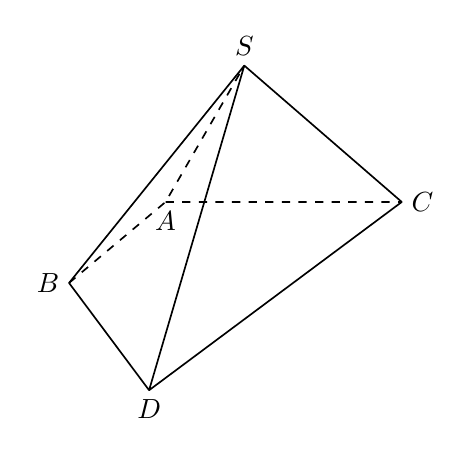
\begin{tikzpicture}
	\coordinate (A) at (0,0) ;
	\coordinate (C) at (3,0) ;
	\coordinate (S) at (60:2) ;
	\coordinate (B) at (-140:1.6) ;
	\coordinate (D) at (-95:2.4) ;
	\draw[semithick,line join=bevel] (B)--(S)--(C)--(D)--cycle (S)--(D) ;
	\draw[semithick,dashed,line join=bevel] (B)--(A)--(S) (A)--(C) ;
	\draw (A) node[below] {$A$}
	(B) node[left] {$B$}
	(C) node[right] {$C$}
	(D) node[below] {$D$}
	(S) node[above] {$S$} ;
\end{tikzpicture}
\end{wrapstuff}

Dans l’espace muni d’un repère orthonormé $\Rijk$ d’unité 1~cm, on considère les points :

\begin{Centrage}
	$A(3;-1;1)$ ; $B(4;-1;0)$ ; $C(0;3;2)$ ; $D(4;3;-2)$ et $S(2;1;4)$.
\end{Centrage}

Dans cet exercice on souhaite montrer que $SABDC$ est une pyramide à base $ABDC$ trapézoïdale de sommet $S$, afin de calculer son volume.

\begin{enumerate}
	\item Montrer que les points $A$, $B$ et $C$ ne sont pas alignés.
	\item 
	\begin{enumerate}
		\item Montrer que les points $A$, $B$, $C$ et $D$ sont coplanaires.
		\item Montrer que le quadrilatère $ABDC$ est un trapèze de bases $[AB]$ et $[CD]$.
		
		\emph{On rappelle qu’un trapèze est un quadrilatère ayant deux côtés opposés parallèles appelés bases.}
	\end{enumerate}
	\item 
	\begin{enumerate}
		\item Démontrer que le vecteur $\Vecteur{n}\begin{pmatrix}2\\1\\2\end{pmatrix}$ est un vecteur normal au plan $(ABC)$.
		\item En déduire une équation cartésienne du plan $(ABC)$.
		\item Déterminer une représentation paramétrique de la droite $\Delta$ passant par le point $S$ et orthogonale au plan $(ABC)$.
		\item On note $I$ le point d’intersection de la droite $\Delta$ et du plan $(ABC)$.
		
		Montrer que le point $I$ a pour coordonnées $\left(\dfrac23;\dfrac13;\dfrac83\right)$, puis montrer que $SI = 2$~cm.
	\end{enumerate}
	\item 
	\begin{enumerate}
		\item Vérifier que le projeté orthogonal $H$ du point $B$ sur la droite $(CD)$ a pour coordonnées $H(3;3;-1)$ et montrer que $HB = 3\sqrt{2}$~cm.
		\item Calculer la valeur exacte de l’aire du trapèze $ABDC$.
		
		On rappelle que l’aire d’un trapèze est donnée par la formule \[ \mathcal{A} = \frac{b+B}{2} \times h \]
		où $b$ et $B$ sont les longueurs des bases du trapèze et $h$ sa hauteur.
	\end{enumerate}
	\item Déterminer le volume de la pyramide $SABDC$.
	
	On rappelle que le volume V d’une pyramide est donné par la formule \[ \mathcal{V} = \frac13 \times \text{aire de la base} \times \text{hauteur}. \]
\end{enumerate}